\begin{figure}[htbp]
\centering
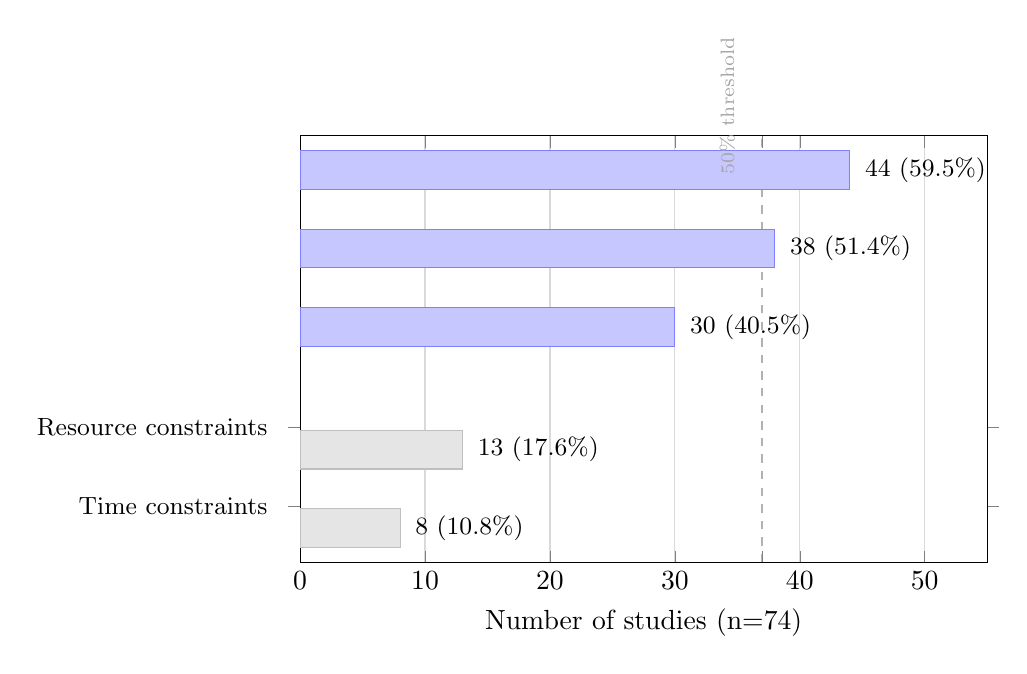
\begin{tikzpicture}
\begin{axis}[
    width=0.85\textwidth,
    height=7cm,
    xbar,
    xlabel={Number of studies (n=74)},
    symbolic y coords={
      {Time constraints},
      {Resource constraints},
      {Technical/Infrastructure},
      {Pedagogical/Curriculum},
      {Student-related}
    },
    ytick=data,
    y tick label style={font=\small, anchor=east, xshift=-4pt},
    clip=false,
    nodes near coords={\pgfplotspointmeta},
    nodes near coords align={horizontal},
    nodes near coords style={font=\small, anchor=west, xshift=2pt},
    point meta=explicit symbolic,
    bar width=14pt,
    xmin=0, xmax=55,
    enlarge y limits=0.18,
    xmajorgrids=true,
    ymajorgrids=false,
    grid style={gray!30},
    extra x ticks={37},
    extra x tick labels={},
    extra x tick style={
      grid=major,
      grid style={dashed, gray!60, line width=0.8pt},
    },
]
\addplot[fill=gray!20, draw=gray!50] coordinates {
  (8,{Time constraints}) [8 (10.8\%)]
  (13,{Resource constraints}) [13 (17.6\%)]
};
\addplot[fill=blue!22, draw=blue!50] coordinates {
  (30,{Technical/Infrastructure}) [30 (40.5\%)]
  (38,{Pedagogical/Curriculum}) [38 (51.4\%)]
  (44,{Student-related}) [44 (59.5\%)]
};
\end{axis}
% 50% threshold annotation
\node[font=\scriptsize, text=gray!70, anchor=south, rotate=90]
  at (5.65, 5.8) {50\% threshold};
\end{tikzpicture}
\caption{Frequency distribution of implementation barrier categories across the 74-study corpus. The dashed line marks the 50\% threshold (n=37): student-related and pedagogical barriers constitute majority challenges, while resource and time constraints are reported by a minority of studies.}
\label{fig:barrier-frequency}
\end{figure}
